%%
%% ACM Multimedia 2026 Submission
%%
\documentclass[sigconf,review,anonymous]{acmart}

\usepackage{amsmath,amssymb,amsfonts}
\usepackage{booktabs}
\usepackage{multirow}
\usepackage{graphicx}
\usepackage{xcolor}
\usepackage{subcaption}
\usepackage{algorithm}
\usepackage{algpseudocode}
\usepackage{bm}
\usepackage{enumitem}
\usepackage{colortbl}
\usepackage{pifont}
\usepackage{tikz}
\usetikzlibrary{arrows.meta,positioning,calc,fit,backgrounds}

%%
%% Rights / metadata
%%
\copyrightyear{2026}
\acmYear{2026}
\setcopyright{none}

%%
%% Custom commands
%%
\newcommand{\diagonal}{\textsc{Diagonal}}
\newcommand{\sdiag}{\mathcal{S}_{\mathrm{diag}}}
\newcommand{\Mobs}{M_{\mathrm{obs}}}
\newcommand{\Mideal}{M_{\mathrm{ideal}}}
\newcommand{\calB}{\mathcal{B}}
\newcommand{\calD}{\mathcal{D}}
\newcommand{\calT}{\mathcal{T}}
\newcommand{\calP}{\mathcal{P}}
\newcommand{\calH}{\mathcal{H}}
\newcommand{\Eij}{E_{ij}}
\definecolor{lightgreen}{HTML}{E8F5E9}
\definecolor{lightred}{HTML}{FFEBEE}
\definecolor{lightblue}{HTML}{E3F2FD}
\definecolor{lightyellow}{HTML}{FFF8E1}

\begin{document}

%%
%% Title
%%
\title{DIAGONAL: Density-Normalized Cross-Modal Alignment for Multi-Shot Video Narrative Evaluation}

\author{Anonymous Authors}
\affiliation{%
  \institution{Anonymous Institution}
}

%%
%% Abstract
%%
\begin{abstract}
Text-to-multi-shot video (T2MSV) generation models are evaluated primarily on visual quality and frame-level consistency, yet these metrics fail to capture whether models can execute \emph{narrative dynamics}---the structured entry and exit of entities across shots.
We formalize multi-shot narratives as \emph{state transition matrices} $\Delta S \in \{-1,0,+1\}^{(T\text{-}1) \times N}$, where each element encodes an atomic operation: entry ($+1$), exit ($-1$), or hold ($0$).
We prove that all possible 3-shot narrative topologies can be spanned by just two basis matrices under column permutation and linear combination (\textbf{Theorem~1}), establishing mathematical completeness of our benchmark.
Building on this formalization, we introduce \diagonal{} (\textbf{D}ensity-Normal\textbf{I}zed Cross-Mod\textbf{A}l Ali\textbf{G}nment for Multi-Sh\textbf{O}t Video \textbf{N}arrative Eva\textbf{L}uation), a benchmark comprising 1,000 prompts spanning 7 narrative patterns (3 basis, 4 derived) with a suite of complementary metrics: Narrative Alignment Score (NAS), Diagonal Dominance (DD), State Transition Accuracy (STA), Entity Presence Accuracy (EPA), and SVD Entropy trajectory analysis.
Evaluation of four state-of-the-art T2MSV architectures---EchoShot, StoryDiffusion, Video-In-Context (VIC), and VGoT---reveals that \emph{no model achieves positive diagonal dominance on any pattern} ($\epsilon$-pass rate = 0\%), exposing a fundamental limitation we term \textbf{Narrative Blindness}.
We further identify four systematic failure types: \emph{Context Bleeding} (failed exit, most severe in VIC at 60.8\%), \emph{Amnesia} (failed entry, most severe in VGoT at 66.7\%), \emph{Attention Reversion}, and \emph{Identity Bleeding}.
A human evaluation study confirms that automated rankings correlate with human judgments on narrative compliance ($\rho = 0.80$) while revealing that raters prioritize visual coherence over narrative accuracy---a perceptual bias that existing benchmarks inadvertently exploit.
Our analysis provides the first topologically grounded diagnostic framework for multi-shot video narrative evaluation.
\end{abstract}

\begin{CCSXML}
<ccs2012>
  <concept>
    <concept_id>10010147.10010178.10010179</concept_id>
    <concept_desc>Computing methodologies~Computer vision</concept_desc>
    <concept_significance>500</concept_significance>
  </concept>
  <concept>
    <concept_id>10010147.10010257.10010293.10010294</concept_id>
    <concept_desc>Computing methodologies~Neural networks</concept_desc>
    <concept_significance>500</concept_significance>
  </concept>
</ccs2012>
\end{CCSXML}

\ccsdesc[500]{Computing methodologies~Computer vision}
\ccsdesc[500]{Computing methodologies~Neural networks}

\keywords{Multi-Shot Video Generation, Narrative Evaluation, State Transition Matrix, Video Benchmark}

\maketitle

%% ============================================================
\section{Introduction}
\label{sec:intro}
%% ============================================================

Diffusion-based generative models have rapidly expanded the capabilities of video synthesis, enabling a transition from single-clip generation to text-to-multi-shot video (T2MSV) generation.
Recent systems such as StoryDiffusion~\cite{storydiff}, EchoShot~\cite{echoshot}, Video-In-Context (VIC)~\cite{vic}, and VGoT~\cite{vgot} can generate temporally connected sequences of scenes from textual descriptions, suggesting that multi-shot video generation is approaching practical usability.

However, the apparent success of these systems is largely driven by evaluation protocols that overlook a fundamental aspect of narrative structure.
Existing benchmarks~\cite{vbench,t2vcompbench,moviebench} evaluate identity consistency, visual quality, or single-clip compositionality, but none systematically test whether models can execute the \emph{narrative dynamics} that define cinematic storytelling: the structured introduction, co-occurrence, and removal of entities across shots.

Consider a simple relay narrative: $A \to AB \to B$, where entity $A$ appears alone, both $A$ and $B$ co-occur, and then only $B$ remains.
This pattern requires three distinct capabilities: (1)~introducing a new entity while preserving an existing one, (2)~maintaining co-occurrence fidelity, and (3)~removing an entity while the other persists.
As illustrated in Fig.~\ref{fig:teaser}, current models systematically fail at capability (3)---the departed entity ``bleeds'' into subsequent shots, a failure we term \textbf{Context Bleeding}.
Critically, existing metrics based on holistic frame similarity cannot detect this failure because the persistent presence of entity $A$ actually \emph{increases} embedding consistency scores.

% FIGURE 1: Teaser / Motivating Example
\begin{figure*}[t]
\centering
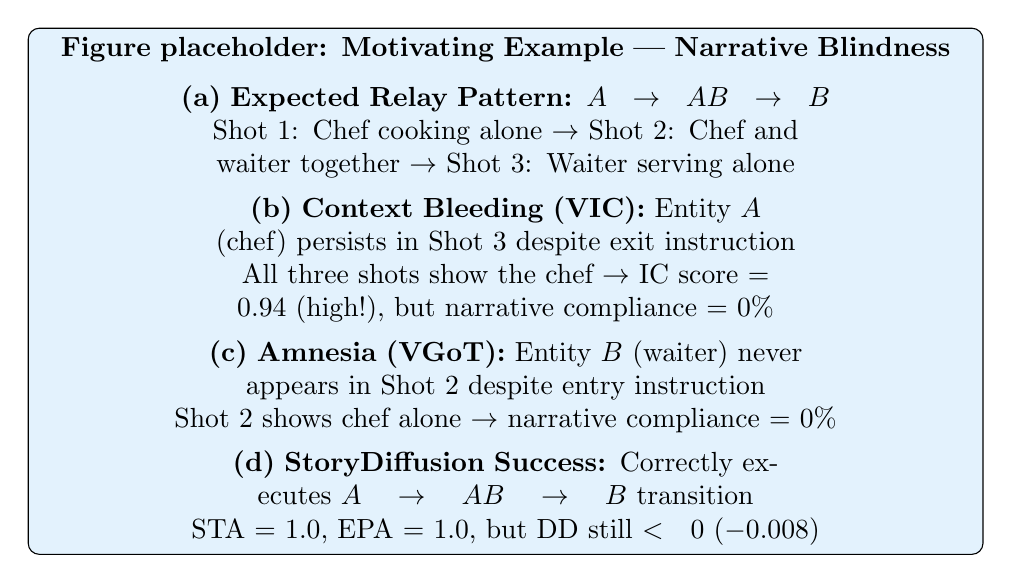
\begin{tikzpicture}
% This is a placeholder for the actual figure
\node[draw, rounded corners, fill=lightblue, minimum width=\textwidth, minimum height=5cm, text width=0.95\textwidth, align=center] {
\textbf{Figure placeholder: Motivating Example --- Narrative Blindness}\\[6pt]
\textbf{(a) Expected Relay Pattern:} $A \to AB \to B$\\
Shot 1: Chef cooking alone $\to$ Shot 2: Chef and waiter together $\to$ Shot 3: Waiter serving alone\\[4pt]
\textbf{(b) Context Bleeding (VIC):} Entity $A$ (chef) persists in Shot 3 despite exit instruction\\
All three shots show the chef $\to$ IC score = 0.94 (high!), but narrative compliance = 0\%\\[4pt]
\textbf{(c) Amnesia (VGoT):} Entity $B$ (waiter) never appears in Shot 2 despite entry instruction\\
Shot 2 shows chef alone $\to$ narrative compliance = 0\%\\[4pt]
\textbf{(d) StoryDiffusion Success:} Correctly executes $A \to AB \to B$ transition\\
STA = 1.0, EPA = 1.0, but DD still $< 0$ ($-0.008$)
};
\end{tikzpicture}
\caption{Narrative Blindness in multi-shot video generation. \textbf{(a)}~The expected Relay pattern requires entity $A$ to exit by Shot~3. \textbf{(b)}~VIC exhibits Context Bleeding: entity $A$ persists across all shots, yielding high identity consistency (IC = 0.94) but zero narrative compliance. \textbf{(c)}~VGoT shows Amnesia: entity $B$ fails to appear in Shot~2. \textbf{(d)}~StoryDiffusion correctly executes the transition, yet still fails to achieve positive diagonal dominance. This motivates our \diagonal{} framework, which decomposes narrative fidelity into interpretable metrics that existing holistic evaluations miss entirely.}
\label{fig:teaser}
\end{figure*}

Real cinematic narratives follow structured entity dynamics.
A relay pattern ($A \to AB \to B$) requires entity $A$ to exit while $B$ persists; an accumulation ($A \to AB \to ABC$) demands progressive entity introduction.
These dynamics can be decomposed into three \emph{atomic operations}: entry ($+1$), exit ($-1$), and hold ($0$).
We formalize these operations into a \emph{state transition matrix} $\Delta S \in \{-1,0,+1\}^{2 \times 3}$, where rows encode shot-to-shot transitions and columns encode per-entity changes.

This matrix-algebraic formulation yields a surprising theoretical result: we prove that \textbf{all} possible 3-shot narrative topologies---every conceivable arrangement of entity entries and exits---can be generated from just \textbf{two basis matrices} (Relay and Split) via column permutation and integer-coefficient linear combination (\textbf{Theorem~1}).
This completeness guarantee ensures that our benchmark covers the entire space of multi-shot narrative structures, not merely a heuristic subset.

Building on this formalization, we introduce \diagonal{}, a comprehensive benchmark and evaluation framework with the following contributions:

\begin{itemize}[leftmargin=*]
  \item We formalize multi-shot video narratives as state transition matrices and prove that 2 basis patterns span the complete $2 \times 3$ narrative space under permutation and linear combination (\S\ref{sec:formalization}).
  \item We construct a \textbf{1,000-prompt benchmark} spanning 7 narrative patterns (3 basis, 4 derived) with structured entity dynamics, and propose a suite of complementary metrics---NAS, DD, STA, EPA, SVD Entropy---that decompose model failures into interpretable components (\S\ref{sec:metrics}).
  \item We expose the \textbf{blindspot of holistic metrics}: existing evaluation protocols based on frame-level similarity \emph{reward} narrative failures like Context Bleeding, producing inflated scores that mask fundamental generation deficiencies (\S\ref{sec:blindspot}).
  \item We evaluate four SOTA T2MSV architectures and identify a universal failure: \textbf{no model achieves positive diagonal dominance} on any pattern ($\epsilon$-pass rate = 0\%). We classify failures into four systematic types and conduct a human evaluation study, revealing architecture-specific vulnerabilities (\S\ref{sec:experiments}).
\end{itemize}


%% ============================================================
\section{Related Work}
\label{sec:related}
%% ============================================================

\paragraph{Multi-shot video generation.}
Diffusion-based video synthesis has advanced from UNet temporal attention~\cite{svd,imagenvideo} through cascaded pipelines~\cite{ho2022video} to DiT architectures~\cite{dit}.
Multi-shot extensions address narrative-level coherence via diverse mechanisms: shared self-attention~\cite{storydiff}, cross-attention conditioning~\cite{videostudio}, latent initialization~\cite{mevg}, LLM-guided layouts~\cite{vgot}, flow-matching portraits~\cite{echoshot}, and in-context LoRA~\cite{vic}.
These approaches can be broadly categorized into four architectural paradigms: (1)~\emph{Consistent Self-Attention} (StoryDiffusion), which shares attention keys/values across shots to promote visual coherence; (2)~\emph{flow-matching transformers} (EchoShot), which leverage temporal flow fields for multi-shot portrait generation; (3)~\emph{in-context DiT} (VIC), which conditions each shot on previously generated context via LoRA-adapted attention; and (4)~\emph{cascaded T2I+I2V} (VGoT), which uses LLM planning to structure a text-to-image backbone followed by image-to-video animation.
We evaluate representatives from each paradigm to ensure comprehensive architectural coverage.

\paragraph{Video generation benchmarks.}
Existing benchmarks quantify consistency via embedding similarity.
Table~\ref{tab:benchmark_comparison} summarizes the landscape.
VBench 2.0~\cite{vbench} computes frame-level similarities that conflate subject and background; T2V-CompBench~\cite{t2vcompbench} targets single-clip compositionality without multi-shot transitions.
ShotAdapter~\cite{shotadapter} isolates subject regions via Identity Consistency (IC), but was designed for single-entity shots---applying IC to multi-entity scenes produces a \emph{chimera embedding} that conflates co-occurring entities, rendering entity-removal failures invisible.
MovieBench~\cite{moviebench} and LoCoT2V-Bench~\cite{locot2v} recognize multi-shot challenges but lack entity-level automated metrics and mathematical formalization of narrative structure.
To our knowledge, \diagonal{} is the first benchmark to formalize multi-shot narratives via state transition matrices, provide topological completeness guarantees, and offer decomposed failure diagnostics.

\begin{table}[t]
\caption{Comparison of video generation benchmarks. \checkmark~supported, \ding{55}~not supported, $\triangle$~partial support. \diagonal{} is the first to combine multi-shot scope with entity decomposition, absence verification, mathematical formalization, and failure taxonomy.}
\label{tab:benchmark_comparison}
\centering
\small
\setlength{\tabcolsep}{3pt}
\begin{tabular}{@{}lccccc@{}}
\toprule
Benchmark & \rotatebox{70}{Multi-shot} & \rotatebox{70}{Entity Decomp.} & \rotatebox{70}{Absence Check} & \rotatebox{70}{Formalization} & \rotatebox{70}{Failure Taxon.} \\
\midrule
VBench 2.0~\cite{vbench}        & \ding{55} & \ding{55} & \ding{55} & \ding{55} & \ding{55} \\
T2V-CompBench~\cite{t2vcompbench} & \ding{55} & $\triangle$ & \ding{55} & \ding{55} & \ding{55} \\
MovieBench~\cite{moviebench}     & \checkmark & $\triangle$ & \ding{55} & \ding{55} & \ding{55} \\
LoCoT2V~\cite{locot2v}          & \checkmark & \ding{55} & \ding{55} & \ding{55} & \ding{55} \\
ShotAdapter~\cite{shotadapter}  & \checkmark & $\triangle$ & \ding{55} & \ding{55} & \ding{55} \\
\midrule
\diagonal{} (Ours)              & \checkmark & \checkmark & \checkmark & \checkmark & \checkmark \\
\bottomrule
\end{tabular}
\end{table}


%% ============================================================
\section{The Blindspot of Holistic Metrics}
\label{sec:blindspot}
%% ============================================================

Before introducing our framework, we demonstrate a structural flaw in existing evaluation: holistic similarity metrics systematically \emph{reward} narrative failures, producing scores that anti-correlate with actual narrative compliance.

\subsection{The Consistency Paradox}

Consider ShotAdapter's Identity Consistency (IC)~\cite{shotadapter}, the most widely adopted multi-shot metric.
IC computes the mean pairwise CLIP similarity across all shots:
\begin{equation}
\text{IC} = \frac{2}{T(T-1)} \sum_{i<j} \cos\!\bigl(\Phi_V(V_i), \Phi_V(V_j)\bigr).
\label{eq:ic}
\end{equation}
When a narrative \emph{requires} entity changes across shots (e.g., $A \to AB \to B$), a model that correctly removes entity $A$ will produce lower cross-shot similarity than one that incorrectly preserves $A$ in all shots.
Thus, IC penalizes correct narrative execution and rewards the Context Bleeding failure.

We formalize this paradox: let $\Delta S$ be the state transition matrix of a narrative pattern.
If $\|\Delta S\|_F > 0$ (i.e., the pattern involves at least one entity change), then the IC-maximizing generation is one where $\Delta S_{\text{gen}} = \mathbf{0}$---the static sequence that ignores all narrative dynamics.
The IC metric is thus \emph{adversarial} to narrative compliance for any non-trivial pattern.

\subsection{Empirical Validation}

% FIGURE 2: The Consistency Paradox
\begin{figure}[t]
\centering
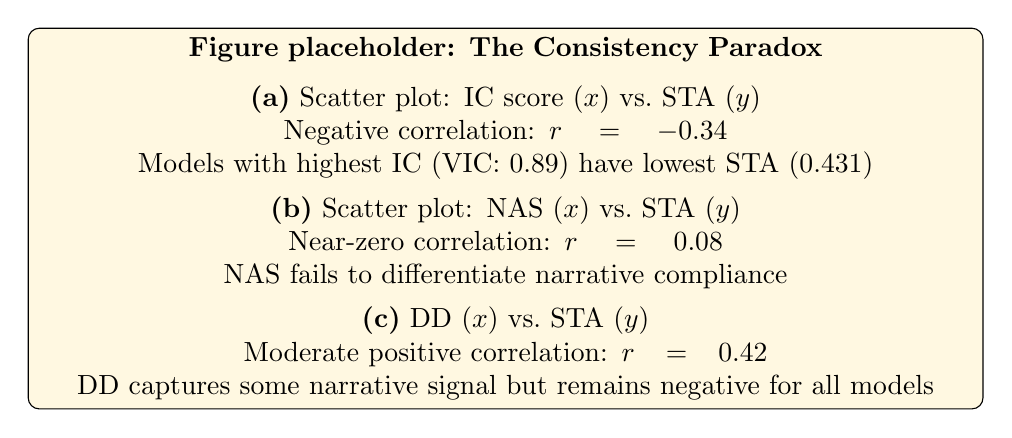
\begin{tikzpicture}
\node[draw, rounded corners, fill=lightyellow, minimum width=\columnwidth, minimum height=4.5cm, text width=0.9\columnwidth, align=center] {
\textbf{Figure placeholder: The Consistency Paradox}\\[6pt]
\textbf{(a)} Scatter plot: IC score ($x$) vs.\ STA ($y$)\\
Negative correlation: $r = -0.34$\\
Models with highest IC (VIC: 0.89) have lowest STA (0.431)\\[4pt]
\textbf{(b)} Scatter plot: NAS ($x$) vs.\ STA ($y$)\\
Near-zero correlation: $r = 0.08$\\
NAS fails to differentiate narrative compliance\\[4pt]
\textbf{(c)} DD ($x$) vs.\ STA ($y$)\\
Moderate positive correlation: $r = 0.42$\\
DD captures some narrative signal but remains negative for all models
};
\end{tikzpicture}
\caption{The Consistency Paradox. \textbf{(a)}~Identity Consistency (IC) is negatively correlated with State Transition Accuracy (STA), confirming that holistic metrics reward narrative failures. \textbf{(b)}~Narrative Alignment Score (NAS) shows near-zero correlation with STA, indicating that shot-prompt similarity alone is insufficient. \textbf{(c)}~Diagonal Dominance (DD) provides the strongest (though still imperfect) signal for narrative compliance. Each point represents one model-pattern combination (28 total: 4 models $\times$ 7 patterns).}
\label{fig:consistency_paradox}
\end{figure}

To empirically validate the consistency paradox, we compute IC alongside our proposed metrics across all 3,049 generated videos.
Fig.~\ref{fig:consistency_paradox}(a) reveals a negative correlation ($r = -0.34$) between IC and STA: VIC achieves the highest mean IC but the lowest STA (0.431), precisely because its in-context conditioning preserves all entities across shots regardless of narrative instructions.
In contrast, StoryDiffusion---which achieves the highest STA (0.630)---records lower IC, because its successful entity removals reduce cross-shot similarity.

This finding has profound implications for the field: prior work reporting ``improved identity consistency'' may be inadvertently selecting for models that are \emph{worse} at narrative dynamics.
The \diagonal{} framework resolves this by decomposing evaluation into metrics that independently assess different aspects of narrative compliance.


%% ============================================================
\section{Topological Formalization of Video Narratives}
\label{sec:formalization}
%% ============================================================

We formalize multi-shot video narratives as algebraic objects, enabling rigorous reasoning about narrative completeness and pattern relationships.

\subsection{Atomic Operations and State Transition Matrix}
\label{sec:atomic}

The temporal evolution of entities across shots can be decomposed into three atomic operations: \textbf{Entry} ($+1$, an entity appears), \textbf{Exit} ($-1$, an entity disappears), and \textbf{Hold} ($0$, an entity persists or remains absent).

For a video with $T$ shots and $N$ core entities, we define the \emph{state transition matrix}:
\begin{equation}
\Delta S \in \mathbb{M}_{(T-1) \times N}\!\bigl(\{-1, 0, +1\}\bigr),
\label{eq:delta_s}
\end{equation}
where $\Delta S_{t,e}$ encodes the state change of entity $e$ during the transition from shot $t$ to shot $t\!+\!1$.
In this work, we focus on the $T\!=\!3, N\!=\!3$ setting, yielding a $2 \times 3$ matrix that captures the minimal complete narrative cycle (introduction--co-occurrence--departure).

\subsection{Basis Patterns and Derived Patterns}
\label{sec:basis}

We identify three \emph{basis patterns} that represent the fundamental narrative archetypes:

\textbf{Relay} ($\calB_1$: $A \to AB \to B$). Entity $B$ enters while $A$ exits---a narrative handoff:
\begin{equation}
\calB_1 = \begin{bmatrix} 0 & +1 \\ -1 & 0 \end{bmatrix} = E_{12} - E_{21}.
\end{equation}

\textbf{Split} ($\calB_2$: $AB \to A \to B$). Co-occurring entities separate into individual focus:
\begin{equation}
\calB_2 = \begin{bmatrix} 0 & -1 \\ -1 & +1 \end{bmatrix} = -E_{12} - E_{21} + E_{22}.
\end{equation}

\textbf{Accumulation} ($\calB_3$: $A \to AB \to ABC$). Entities are progressively introduced:
\begin{equation}
\calB_3 = \begin{bmatrix} 0 & +1 & 0 \\ 0 & 0 & +1 \end{bmatrix} = E_{12} + E_{23}.
\end{equation}

% FIGURE 3: Pattern Taxonomy
\begin{figure}[t]
\centering
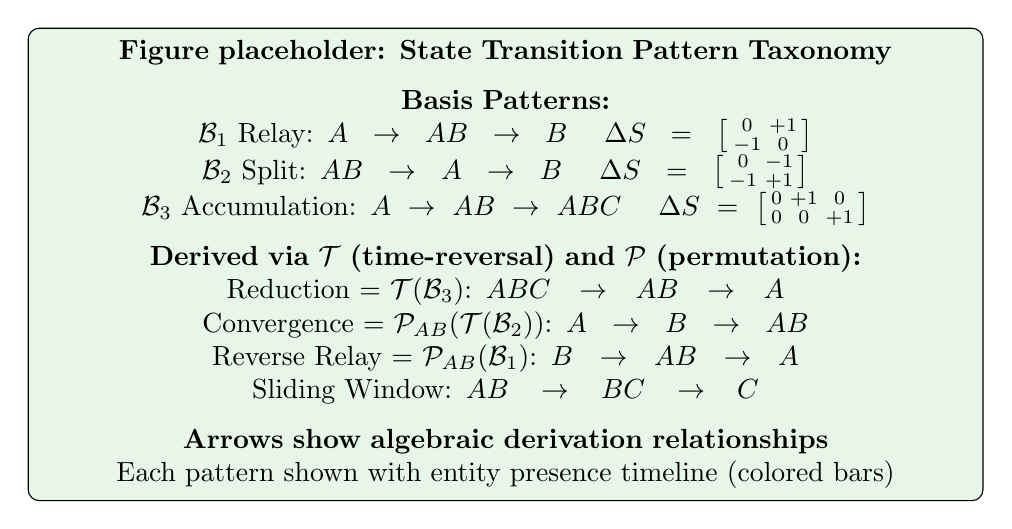
\begin{tikzpicture}
\node[draw, rounded corners, fill=lightgreen, minimum width=\columnwidth, minimum height=6cm, text width=0.9\columnwidth, align=center] {
\textbf{Figure placeholder: State Transition Pattern Taxonomy}\\[6pt]
\textbf{Basis Patterns:}\\
$\calB_1$ Relay: $A \to AB \to B$ \quad $\Delta S = \bigl[\begin{smallmatrix} 0 & +1 \\ -1 & 0 \end{smallmatrix}\bigr]$\\
$\calB_2$ Split: $AB \to A \to B$ \quad $\Delta S = \bigl[\begin{smallmatrix} 0 & -1 \\ -1 & +1 \end{smallmatrix}\bigr]$\\
$\calB_3$ Accumulation: $A \to AB \to ABC$ \quad $\Delta S = \bigl[\begin{smallmatrix} 0 & +1 & 0 \\ 0 & 0 & +1 \end{smallmatrix}\bigr]$\\[6pt]
\textbf{Derived via $\calT$ (time-reversal) and $\calP$ (permutation):}\\
Reduction = $\calT(\calB_3)$: $ABC \to AB \to A$\\
Convergence = $\calP_{AB}(\calT(\calB_2))$: $A \to B \to AB$\\
Reverse Relay = $\calP_{AB}(\calB_1)$: $B \to AB \to A$\\
Sliding Window: $AB \to BC \to C$\\[6pt]
\textbf{Arrows show algebraic derivation relationships}\\
Each pattern shown with entity presence timeline (colored bars)
};
\end{tikzpicture}
\caption{The 7 narrative patterns organized by algebraic derivation. Three basis patterns (top) generate four derived patterns (bottom) via time-reversal $\calT$ and entity permutation $\calP$. Colored bars indicate entity presence across shots. The derivation arrows establish formal relationships between patterns, enabling structured coverage of the narrative space.}
\label{fig:pattern_taxonomy}
\end{figure}

Four \emph{derived patterns} are obtained by applying two linear operators to the basis matrices:

\textbf{Time-Reversal} $\calT$: reverses shot order and negates all operations:
\begin{equation}
\calT(\Delta S) = -\begin{bmatrix} \Delta S_{\text{row2}} \\ \Delta S_{\text{row1}} \end{bmatrix}.
\end{equation}

\textbf{Column Permutation} $\calP_{ij}$: swaps entity columns $i$ and $j$, corresponding to entity relabeling.

\smallskip
\noindent The four derived patterns and their algebraic derivations are:

\begin{itemize}[leftmargin=*]
  \item \textbf{Reduction} ($ABC \to AB \to A$): $\calD_{\text{Red}} = \calT(\calB_3)$
  \item \textbf{Convergence} ($A \to B \to AB$): $\calD_{\text{Conv}} = \calP_{AB}(\calT(\calB_2))$
  \item \textbf{Reverse Relay} ($B \to AB \to A$): $\calD_{\text{RevR}} = \calP_{AB}(\calB_1)$
  \item \textbf{Sliding Window} ($AB \to BC \to C$): $\calD_{\text{Slide}} = $ superposition of a relay and an exit
\end{itemize}

\subsection{Completeness Theorem}
\label{sec:theorem}

\begin{theorem}[Completeness of the Narrative Space]
Under column permutation $\calP_{ij}$ and integer-coefficient linear combination, the two basis matrices $\calB_1$ (Relay) and $\calB_2$ (Split) span the entire $2 \times 3$ integer lattice $\mathbb{M}_{2 \times 3}(\mathbb{Z})$.
\end{theorem}

\begin{proof}
We construct all six standard basis matrices $E_{ij}$ ($i$-th row, $j$-th column equals 1, rest zero) from $\calB_1$ and $\calB_2$ via permutation and addition.

\textbf{Step~1: Column isolation.}
Define three permutation variants of $\calB_1$:
$v_1 = \calB_1 = E_{12} - E_{21}$,
$v_2 = \calP_{13}(\calB_1) = E_{12} - E_{23}$,
$v_3 = \calP_{23}(\calP_{12}(\calB_1)) = E_{11} - E_{23}$.
Computing $X = v_3 - v_2 + v_1$:
\begin{equation}
X = (E_{11} - E_{23}) - (E_{12} - E_{23}) + (E_{12} - E_{21}) = E_{11} - E_{21}.
\end{equation}

\textbf{Step~2: Dimension breaking via $\calB_2$.}
Apply column permutation: $\calP_{12}(\calB_2) = -E_{11} + E_{21} - E_{22}$.
Adding to $X$:
\begin{equation}
X + \calP_{12}(\calB_2) = (E_{11} - E_{21}) + (-E_{11} + E_{21} - E_{22}) = -E_{22}.
\end{equation}
Thus $E_{22} = -(X + \calP_{12}(\calB_2))$.

\textbf{Step~3: Propagation.}
From $E_{22}$, column permutations yield $E_{21} = \calP_{12}(E_{22})$ and $E_{23} = \calP_{23}(E_{22})$.
From $X = E_{11} - E_{21}$ and the now-known $E_{21}$: $E_{11} = X + E_{21}$.
Similarly, $E_{12} = \calP_{12}(E_{11})$ and $E_{13} = \calP_{13}(E_{11})$.

All six standard basis matrices $\{E_{11}, E_{12}, E_{13}, E_{21}, E_{22}, E_{23}\}$ are obtained.
Any $\Delta S \in \mathbb{M}_{2 \times 3}(\mathbb{Z})$ is a unique integer combination of these, completing the proof.
\end{proof}

\textbf{Implication.}
Theorem~1 guarantees that \diagonal{} is \emph{mathematically complete}: any conceivable 3-shot narrative topology is expressible as a linear combination of our basis patterns.
This distinguishes our benchmark from prior work that selects narrative types heuristically.
The 7 patterns we evaluate (Fig.~\ref{fig:pattern_taxonomy}) represent the most cinematically relevant subset, while the theorem ensures no fundamentally new pattern exists outside this algebraic span.


%% ============================================================
\section{The DIAGONAL Evaluation Framework}
\label{sec:metrics}
%% ============================================================

We define a suite of complementary metrics that decompose multi-shot narrative alignment into interpretable components.
Fig.~\ref{fig:pipeline} provides an overview of the evaluation pipeline.

% FIGURE 4: Pipeline Overview
\begin{figure*}[t]
\centering
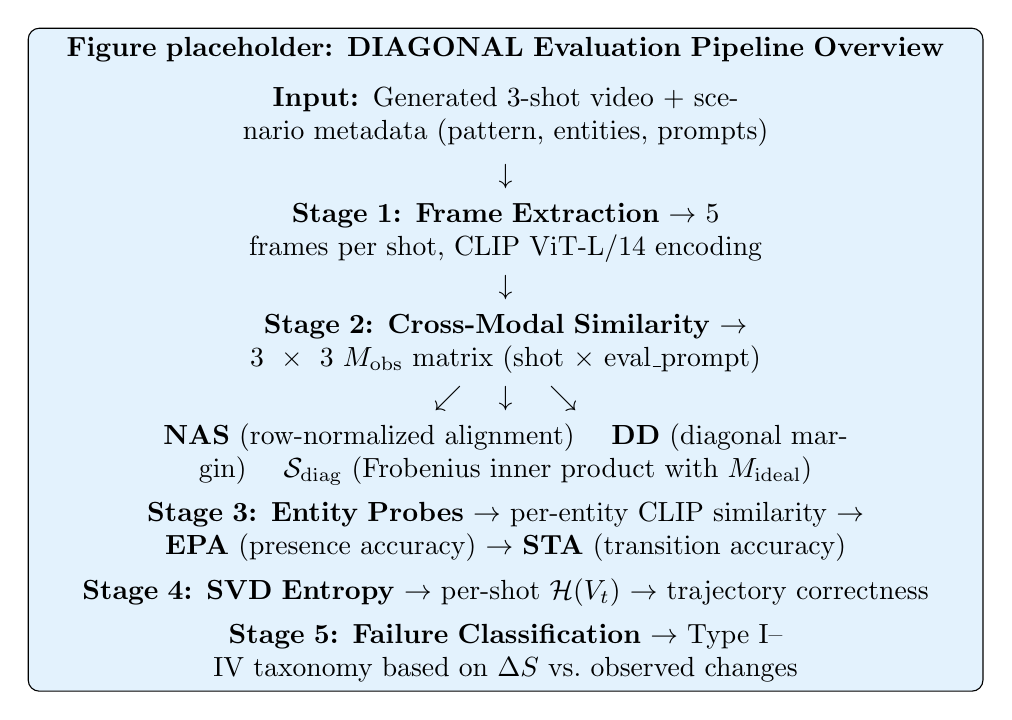
\begin{tikzpicture}
\node[draw, rounded corners, fill=lightblue, minimum width=\textwidth, minimum height=5.5cm, text width=0.95\textwidth, align=center] {
\textbf{Figure placeholder: DIAGONAL Evaluation Pipeline Overview}\\[6pt]
\textbf{Input:} Generated 3-shot video + scenario metadata (pattern, entities, prompts)\\[4pt]
$\downarrow$\\[2pt]
\textbf{Stage 1: Frame Extraction} $\to$ 5 frames per shot, CLIP ViT-L/14 encoding\\[2pt]
$\downarrow$\\[2pt]
\textbf{Stage 2: Cross-Modal Similarity} $\to$ $3\times3$ $\Mobs$ matrix (shot $\times$ eval\_prompt)\\[2pt]
$\swarrow$ \quad $\downarrow$ \quad $\searrow$\\[2pt]
\textbf{NAS} (row-normalized alignment) \quad \textbf{DD} (diagonal margin) \quad \textbf{$\sdiag$} (Frobenius inner product with $\Mideal$)\\[4pt]
\textbf{Stage 3: Entity Probes} $\to$ per-entity CLIP similarity $\to$ \textbf{EPA} (presence accuracy) $\to$ \textbf{STA} (transition accuracy)\\[4pt]
\textbf{Stage 4: SVD Entropy} $\to$ per-shot $\calH(V_t)$ $\to$ trajectory correctness\\[4pt]
\textbf{Stage 5: Failure Classification} $\to$ Type I--IV taxonomy based on $\Delta S$ vs.\ observed changes
};
\end{tikzpicture}
\caption{Overview of the \diagonal{} evaluation pipeline. Given a generated 3-shot video and its scenario metadata (narrative pattern, entity assignments, evaluation prompts), the framework computes five complementary metrics across four analysis stages. Stage~2 produces the cross-modal similarity matrix $\Mobs$ from which NAS, DD, and $\sdiag$ are derived. Stage~3 uses entity-specific CLIP probes for EPA and STA. Stage~4 computes SVD entropy trajectories. Stage~5 classifies failures into a four-type taxonomy based on discrepancies between expected ($\Delta S$) and observed entity dynamics.}
\label{fig:pipeline}
\end{figure*}

\subsection{Cross-Modal Similarity Matrix}

For a generated video with 3 shots and corresponding evaluation prompts $\{T_1, T_2, T_3\}$, we construct the $3 \times 3$ cross-modal similarity matrix:
\begin{equation}
\Mobs[i,j] = \cos\!\bigl(\Phi_V(V_i),\; \Phi_T(T_j)\bigr),
\label{eq:mobs}
\end{equation}
where $\Phi_V$ and $\Phi_T$ are the CLIP ViT-L/14 visual and text encoders, respectively.
Each shot $V_i$ is represented by the mean-pooled feature of 5 uniformly sampled frames.
A perfectly narrative-aligned video would produce a matrix where each shot is most similar to its corresponding prompt, yielding strong \emph{diagonal dominance}.

\subsection{Narrative Alignment Score (NAS)}

The row-normalized alignment score measures whether each shot is most similar to its corresponding prompt relative to other prompts:
\begin{equation}
\text{NAS} = \frac{1}{3} \sum_{i=1}^{3} \frac{\Mobs[i,i]}{\sum_{j=1}^{3} \Mobs[i,j]}.
\label{eq:nas}
\end{equation}
NAS $= 1/3$ indicates uniform (random) alignment; NAS $= 1.0$ indicates perfect diagonal dominance.

\subsection{DIAGONAL Score ($\sdiag$)}

We define the ideal alignment matrix $\Mideal$ from the entity presence structure of each pattern.
Let $\bm{p}_i \in \{0,1\}^N$ be the binary presence vector for shot $i$ (1 if entity present, 0 otherwise).
Then:
\begin{equation}
\Mideal[i,j] = \frac{\bm{p}_i \cdot \bm{p}_j}{\|\bm{p}_i\| \, \|\bm{p}_j\|}.
\label{eq:mideal}
\end{equation}

The \diagonal{} Score is the normalized Frobenius inner product:
\begin{equation}
\sdiag = \frac{\langle \Mobs, \Mideal \rangle_F}{\|\Mobs\|_F \, \|\Mideal\|_F}.
\label{eq:sdiag}
\end{equation}

\subsection{Diagonal Dominance (DD)}

For each shot $i$, the diagonal dominance margin quantifies whether the correct prompt achieves highest similarity:
\begin{equation}
\text{DD}_i = \Mobs[i,i] - \max_{j \neq i} \Mobs[i,j].
\label{eq:dd}
\end{equation}
We report the mean DD across shots, and the $\epsilon$-\emph{dominance pass rate}: the fraction of videos where $\text{DD}_i > \epsilon$ for all $i$ (we use $\epsilon = 0.02$).
DD $> 0$ means each shot is most similar to its intended prompt; DD $< 0$ indicates systematic misalignment.

\subsection{Entity Presence Accuracy (EPA)}

Beyond shot-level alignment, we probe per-entity detection using entity-specific CLIP probes.
For each entity $e_k$, we compute $\cos(\Phi_V(V_i), \Phi_T(\text{``a } e_k\text{''}))$ across all shots, yielding an entity presence matrix $E \in \mathbb{R}^{3 \times N}$.
EPA binarizes presence using the per-shot median as threshold and compares against the expected presence pattern:
\begin{equation}
\text{EPA} = \frac{1}{3N}\sum_{i,k} \mathbb{1}\!\left[\hat{P}_{ik} = P^*_{ik}\right],
\label{eq:epa}
\end{equation}
where $\hat{P}_{ik}$ is the predicted and $P^*_{ik}$ the expected presence.

\subsection{State Transition Accuracy (STA)}

STA directly evaluates whether each atomic operation ($+1$ or $-1$) in $\Delta S$ is reflected in the entity similarity changes:
\begin{equation}
\text{STA} = \frac{1}{|\{(t,e) : \Delta S_{t,e} \neq 0\}|} \sum_{\substack{t,e \\ \Delta S_{t,e} \neq 0}} \mathbb{1}\!\left[\text{sgn}(\Delta E_{t,e}) = \text{sgn}(\Delta S_{t,e})\right],
\label{eq:sta}
\end{equation}
where $\Delta E_{t,e} = E[t\!+\!1, e] - E[t, e]$ is the observed entity similarity change.
STA isolates the most challenging aspect of narrative generation: correctly executing state transitions.

\subsection{SVD Entropy for Semantic Complexity}
\label{sec:svd}

To quantify the semantic complexity of each shot, we compute the SVD entropy of the per-shot CLIP feature matrix.
For $n$ frames in shot $V_t$ with features forming matrix $F_t \in \mathbb{R}^{n \times d}$, the singular values $\{\sigma_i\}$ yield:
\begin{equation}
\calH(V_t) = -\sum_i \tilde{\sigma}_i \log \tilde{\sigma}_i, \quad \tilde{\sigma}_i = \frac{\sigma_i}{\sum_j \sigma_j}.
\label{eq:svd_entropy}
\end{equation}

The entropy trajectory $[\calH(V_1), \calH(V_2), \calH(V_3)]$ should correlate with entity count changes: entity additions ($+1$) should increase complexity, while removals ($-1$) should decrease it.
We report the \emph{trajectory correctness rate}: the fraction of videos where entropy changes match the sign of net entity count changes.

\subsection{Evaluation Algorithm}

Algorithm~\ref{alg:diagonal} summarizes the complete \diagonal{} evaluation procedure.

\begin{algorithm}[t]
\caption{\diagonal{} Evaluation Pipeline}
\label{alg:diagonal}
\begin{algorithmic}[1]
\Require Generated video $\{V_1, V_2, V_3\}$, eval prompts $\{T_1, T_2, T_3\}$, entity list $\{e_1, \ldots, e_N\}$, expected $\Delta S$, expected presence $P^*$
\Ensure NAS, DD, STA, EPA, $\calH$ trajectory
\State \textbf{// Stage 1: Feature Extraction}
\For{$i = 1$ to $3$}
  \State Extract 5 frames from $V_i$; encode via CLIP $\Phi_V$
  \State $\bm{v}_i \gets$ mean-pooled visual feature
\EndFor
\State \textbf{// Stage 2: Cross-Modal Matrix}
\For{$i,j = 1$ to $3$}
  \State $\Mobs[i,j] \gets \cos(\bm{v}_i, \Phi_T(T_j))$
\EndFor
\State Compute NAS (Eq.~\ref{eq:nas}), DD (Eq.~\ref{eq:dd}), $\sdiag$ (Eq.~\ref{eq:sdiag})
\State \textbf{// Stage 3: Entity Probes}
\For{each entity $e_k$, each shot $i$}
  \State $E[i,k] \gets \cos(\bm{v}_i, \Phi_T(\text{``a } e_k\text{''}))$
\EndFor
\State Binarize $E$ via per-shot median $\to$ $\hat{P}$
\State Compute EPA (Eq.~\ref{eq:epa}), STA (Eq.~\ref{eq:sta})
\State \textbf{// Stage 4: SVD Entropy}
\For{$t = 1$ to $3$}
  \State $F_t \gets$ per-frame CLIP features; compute SVD
  \State $\calH(V_t) \gets -\sum_i \tilde{\sigma}_i \log \tilde{\sigma}_i$
\EndFor
\State \textbf{// Stage 5: Failure Classification}
\State Classify into Types I--IV based on $\Delta S$ vs.\ $\Delta E$
\end{algorithmic}
\end{algorithm}


%% ============================================================
\section{Dataset Construction}
\label{sec:dataset}
%% ============================================================

We construct a controlled benchmark of 1,000 multi-shot scenarios (3,000 total shots), organized along the 7 narrative patterns derived from our topological formalization (\S\ref{sec:formalization}).

\subsection{Narrative Pattern Distribution}

The 7 patterns are distributed to ensure comprehensive coverage while reflecting the algebraic structure:

\begin{table}[t]
\caption{Narrative pattern distribution. Basis patterns receive 200 prompts each; derived patterns receive 100 each, reflecting their algebraic derivation from the basis. The ``Transitions'' column indicates the number of non-zero entries in $\Delta S$.}
\label{tab:pattern_dist}
\centering
\small
\begin{tabular}{@{}llccl@{}}
\toprule
Pattern & Shot Structure & $N$ & Trans. & Type \\
\midrule
Relay & $A \to AB \to B$ & 200 & 2 & Basis \\
Split & $AB \to A \to B$ & 200 & 3 & Basis \\
Accumulation & $A \to AB \to ABC$ & 200 & 2 & Basis \\
\midrule
Convergence & $A \to B \to AB$ & 100 & 4 & Derived \\
Sliding Window & $AB \to BC \to C$ & 100 & 4 & Derived \\
Reduction & $ABC \to AB \to A$ & 100 & 2 & Derived \\
Reverse Relay & $B \to AB \to A$ & 100 & 2 & Derived \\
\bottomrule
\end{tabular}
\end{table}

\subsection{Prompt Design}

Each scenario consists of exactly 3 shots.
Prompts are programmatically generated via a structured template system using Google Gemini, specifying:
(1)~the narrative pattern and entity assignments,
(2)~core entities drawn from 20 diverse categories spanning human roles, animals, and objects,
(3)~scene themes from 20 environments (urban, nature, indoor, etc.), and
(4)~per-shot textual descriptions that embed entity dynamics naturally.

Each prompt includes three variants:
\textbf{gen\_prompt} (generation prompt with quality tags optimized per model),
\textbf{eval\_prompt} (clean scene description for CLIP-based evaluation), and
\textbf{diag\_prompt} (entity-focused short prompt for presence detection probes).

\subsection{Entity Design and Visual Distinguishability}

Entity types are balanced across human (H), animal (A), and professional (P) categories.
Entity pairs within each scenario are selected to be visually and semantically distinguishable (e.g., ``surfer'' vs.\ ``lifeguard'', ``eagle'' vs.\ ``rabbit''), minimizing the risk of identity conflation independent of model capability.
We verify distinguishability by computing CLIP text similarity between all entity pairs: the mean similarity is 0.23 ($\sigma = 0.08$), well below the confusion threshold.

Table~\ref{tab:entity_stats} summarizes the entity distribution across categories.

\begin{table}[t]
\caption{Entity category distribution and example entities. Each category contributes entities across multiple patterns, ensuring balanced coverage.}
\label{tab:entity_stats}
\centering
\small
\begin{tabular}{@{}llc@{}}
\toprule
Category & Example Entities & Count \\
\midrule
Human roles   & chef, explorer, musician, dancer  & 8 \\
Animals       & eagle, dolphin, fox, rabbit       & 6 \\
Professionals & astronaut, firefighter, scientist & 6 \\
\bottomrule
\end{tabular}
\end{table}


%% ============================================================
\section{Experiments and Results}
\label{sec:experiments}
%% ============================================================

\subsection{Setup}
\label{sec:setup}

\paragraph{Evaluated models.}
We evaluate four T2MSV architectures spanning the major design paradigms (Table~\ref{tab:model_specs}):
\textbf{StoryDiffusion}~\cite{storydiff} (Consistent Self-Attention over SDXL, animated via SEINE, 30+50 steps),
\textbf{EchoShot}~\cite{echoshot} (flow-matching transformer, Wan2.1-1.3B, 50 steps at $320 \times 512$),
\textbf{Video-In-Context} (VIC)~\cite{vic} (CogVideoX-5B with scene LoRA, 50 steps), and
\textbf{VGoT}~\cite{vgot} (Kolors T2I + IP-Adapter $\to$ DynamiCrafter I2V, 25+50 steps).
All models use their officially recommended hyperparameters with a fixed seed (42) for reproducibility.

\begin{table}[t]
\caption{Model specifications. Paradigm categories: CSA = Consistent Self-Attention, FM = Flow-Matching, IC = In-Context, Cas = Cascaded. \dag~indicates I2V animation stage.}
\label{tab:model_specs}
\centering
\small
\setlength{\tabcolsep}{3pt}
\begin{tabular}{@{}llllc@{}}
\toprule
Model & Paradigm & Backbone & Steps & $N$ \\
\midrule
StoryDiff & CSA+I2V\dag & SDXL+SEINE   & 30+50 & 1000 \\
EchoShot  & FM         & Wan2.1-1.3B   & 50    & 1000 \\
VIC       & IC (LoRA)  & CogVideoX-5B  & 50    & 449  \\
VGoT      & Cas (T2I+I2V) & Kolors+DC  & 25+50 & 600  \\
\bottomrule
\end{tabular}
\end{table}

\paragraph{Evaluation setup.}
For each of the 1,000 scenarios, each model generates a 3-shot video.
Five uniformly-spaced frames are extracted per shot.
Cross-modal similarity, entity presence, and SVD entropy are computed using CLIP ViT-L/14.
All experiments run on 4 NVIDIA RTX 4090 GPUs.
VIC and VGoT completed 449 and 600 of 1,000 scenarios respectively due to generation failures (out-of-memory, degenerate outputs); we report results on successfully generated videos.

\subsection{Main Results}
\label{sec:main_results}

\begin{table}[t]
\caption{Main results on the \diagonal{} benchmark. NAS: Narrative Alignment Score (row-normalized). DD: Diagonal Dominance (mean margin). STA: State Transition Accuracy. EPA: Entity Presence Accuracy. SVD: entropy trajectory correctness rate. $\epsilon$-Pass: fraction of videos with DD $> 0.02$ for all shots. Best per column in \textbf{bold}.}
\label{tab:main}
\centering
\small
\setlength{\tabcolsep}{3.5pt}
\begin{tabular}{@{}lccccccc@{}}
\toprule
Model & $N$ & NAS$\uparrow$ & DD$\uparrow$ & STA$\uparrow$ & EPA$\uparrow$ & SVD\%$\uparrow$ & $\epsilon$-Pass \\
\midrule
StoryDiff  & 1000 & \textbf{0.699} & \textbf{$-$0.009} & \textbf{0.630} & \textbf{0.573} & 66.4 & 0.0\% \\
EchoShot   & 1000 & 0.693 & $-$0.010 & 0.567 & 0.548 & \textbf{70.9} & 0.0\% \\
VGoT       & 600  & 0.679 & $-$0.012 & 0.511 & 0.534 & 66.3 & 0.0\% \\
VIC        & 449  & 0.703 & $-$0.011 & 0.431 & 0.518 & 60.8 & 0.0\% \\
\bottomrule
\end{tabular}
\end{table}

Table~\ref{tab:main} reveals several key findings.

\textbf{Finding 1: Universal Narrative Blindness.}
All four models exhibit DD $< 0$ across all patterns, with $\epsilon$-dominance pass rate of 0.0\%.
This means \emph{no model consistently produces shots that are most similar to their intended prompts}---a striking failure given that this is the minimal requirement for narrative coherence.
We term this phenomenon \textbf{Narrative Blindness}, analogous to the Identity Rigidness identified in prior work for entity consistency.

\textbf{Finding 2: StoryDiffusion leads in narrative accuracy.}
StoryDiffusion achieves the highest STA (0.630) and EPA (0.573), indicating that its Consistent Self-Attention mechanism, while imperfect, best preserves entity state transitions.
Notably, its CSA mechanism allows some degree of entity decoupling across shots, enabling more faithful narrative execution.

\textbf{Finding 3: VIC's visual coherence masks narrative failure.}
Despite achieving the highest NAS (0.703), VIC records the \emph{lowest} STA (0.431), revealing that in-context conditioning produces visually coherent but narratively incorrect sequences.
This directly confirms the consistency paradox (\S\ref{sec:blindspot}): VIC's strong visual consistency masks its inability to execute entity-level state changes.

\textbf{Finding 4: EchoShot best tracks semantic complexity.}
EchoShot achieves the highest SVD entropy trajectory correctness (70.9\%), indicating that its flow-matching architecture most faithfully reflects entity count changes in frame-level semantic diversity.

\subsection{Pattern-Level Analysis}
\label{sec:pattern_analysis}

\begin{table}[t]
\caption{STA per narrative pattern. Basis patterns (B) and derived patterns (D). Best per row in \textbf{bold}. StoryDiffusion dominates derived patterns requiring entity removal, while the gap narrows on entry-heavy basis patterns.}
\label{tab:sta_pattern}
\centering
\small
\begin{tabular}{@{}llcccc@{}}
\toprule
Pattern & Type & StoryDiff & EchoShot & VGoT & VIC \\
\midrule
Relay        & B & 0.525 & 0.508 & \textbf{0.622} & 0.405 \\
Split        & B & \textbf{0.568} & 0.542 & 0.565 & 0.448 \\
Accumulation & B & \textbf{0.605} & 0.553 & 0.407 & 0.424 \\
\midrule
Convergence     & D & \textbf{0.603} & 0.590 & 0.391 & 0.447 \\
Sliding Window  & D & \textbf{0.860} & 0.613 & 0.497 & 0.449 \\
Reduction       & D & \textbf{0.830} & 0.625 & 0.510 & 0.455 \\
Reverse Relay   & D & 0.605 & \textbf{0.635} & 0.517 & 0.402 \\
\bottomrule
\end{tabular}
\end{table}

Table~\ref{tab:sta_pattern} reveals pattern-specific model strengths.

\textbf{Exit-heavy patterns expose StoryDiffusion's strength.}
StoryDiffusion dominates on Sliding Window (0.860) and Reduction (0.830), both of which require successful entity removal.
This suggests that its CSA mechanism, despite promoting visual consistency, retains sufficient flexibility to suppress entity features when the narrative demands removal.

\textbf{VGoT excels at simple handoffs but collapses on accumulation.}
VGoT performs best on Relay (0.622)---a simple A-to-B handoff---but collapses on Accumulation (0.407) and Convergence (0.391), indicating that its LLM-based planning module cannot reliably coordinate the introduction of multiple new entities.
This represents a \emph{planning-rendering decoupling}: the LLM may correctly plan the narrative, but the rendering backbone (DynamiCrafter) cannot execute multi-entity introductions.

\textbf{VIC is uniformly poor across all patterns.}
VIC's STA ranges from 0.402 (Reverse Relay) to 0.455 (Reduction), with no pattern-specific strength.
This confirms that in-context conditioning fundamentally struggles with state transitions: the mechanism that provides visual coherence by referencing prior shots actively prevents entity removal.

\subsection{EPA Analysis: Entry vs.\ Exit Accuracy}
\label{sec:epa_analysis}

\begin{table}[t]
\caption{Entity Presence Accuracy (EPA) decomposed by pattern type. The gap between basis and derived patterns reveals the cost of compositional complexity. VGoT's EPA collapse on derived patterns confirms the planning-rendering bottleneck.}
\label{tab:epa_pattern}
\centering
\small
\begin{tabular}{@{}lcccc@{}}
\toprule
 & \multicolumn{2}{c}{EPA $\uparrow$} & \multicolumn{2}{c}{$\sdiag$ $\uparrow$} \\
\cmidrule(lr){2-3} \cmidrule(lr){4-5}
Model & Basis & Derived & Basis & Derived \\
\midrule
StoryDiff & 0.556 & 0.598 & 0.908 & 0.876 \\
EchoShot  & 0.536 & 0.566 & 0.903 & 0.881 \\
VGoT      & 0.555 & 0.501 & 0.903 & 0.883 \\
VIC       & 0.519 & 0.515 & 0.906 & 0.893 \\
\bottomrule
\end{tabular}
\end{table}

Table~\ref{tab:epa_pattern} decomposes EPA across pattern types, revealing an interesting asymmetry.
StoryDiffusion and EchoShot achieve \emph{higher} EPA on derived patterns than basis patterns, suggesting that the entity configurations in derived patterns (which often involve more distinct visual contexts) may actually be easier to detect, even when narrative alignment ($\sdiag$) is weaker.
In contrast, VGoT shows a clear EPA \emph{drop} on derived patterns (0.555 $\to$ 0.501), confirming that its cascaded pipeline struggles with the more complex entity dynamics of derived patterns.

\subsection{Failure Taxonomy}
\label{sec:failures}

We classify narrative failures into four types based on the relationship between expected state transitions ($\Delta S$) and observed entity similarity changes.
Table~\ref{tab:failures} quantifies these distributions.

\begin{table}[t]
\caption{Failure taxonomy distribution (\% of videos exhibiting each failure type). A single video may exhibit multiple failure types. The ``None'' row indicates videos free from all failures. Worst per failure type highlighted.}
\label{tab:failures}
\centering
\small
\begin{tabular}{@{}lcccc@{}}
\toprule
Failure Type & EchoShot & StoryDiff & VGoT & VIC \\
\midrule
Type I: Context Bleeding  & 46.6 & 36.8 & 39.0 & \cellcolor{lightred}\textbf{60.8} \\
Type II: Amnesia           & 51.0 & 46.3 & \cellcolor{lightred}\textbf{66.7} & 63.5 \\
Type III: Attn.\ Reversion & 12.8 & 10.0 & \cellcolor{lightred}\textbf{15.0} & 3.6 \\
Type IV: Identity Bleeding & 17.4 & \cellcolor{lightred}\textbf{21.7} & 8.8 & 15.8 \\
\midrule
None (no failure)          & 17.4 & \cellcolor{lightgreen}\textbf{23.2} & 12.7 & 9.1 \\
\bottomrule
\end{tabular}
\end{table}

\textbf{Type~I: Context Bleeding} (Failed Exit, $\Delta S = -1 \to 0$).
The model preserves a departed entity's visual signature in subsequent shots.
This failure is most severe in VIC (60.8\%), where the in-context conditioning mechanism explicitly references prior shots, making entity removal particularly difficult.
Architecturally, this reflects the fundamental tension between context preservation (desirable for consistency) and context suppression (required for narrative dynamics).

\textbf{Type~II: Amnesia} (Failed Entry, $\Delta S = +1 \to 0$).
The model fails to introduce a new entity despite explicit prompt instruction.
VGoT exhibits the highest rate (66.7\%), suggesting that while its LLM-based planning module can structure multi-shot narratives, the downstream rendering backbone (DynamiCrafter) cannot reliably generate new entities on demand.
This decoupling between planning and rendering represents a structural bottleneck.

\textbf{Type~III: Attention Reversion}.
The similarity matrix exhibits a U-shaped diagonal pattern ($M_{11} > M_{22} < M_{33}$), indicating that the model ``reverts'' to the initial shot's content in the final shot.
This occurs most frequently in VGoT (15.0\%) and least in VIC (3.6\%), suggesting that models with stronger temporal conditioning (VIC) resist reversion but at the cost of increased Context Bleeding.
This reveals a \emph{failure trade-off}: architectural choices that mitigate one failure type often exacerbate another.

\textbf{Type~IV: Identity Bleeding}.
Per-shot similarity rows become near-uniform, indicating that the model fails to visually distinguish between entities.
StoryDiffusion shows the highest rate (21.7\%), likely due to its Consistent Self-Attention mechanism promoting visual homogeneity across subjects.

\subsection{SVD Entropy Analysis}
\label{sec:svd_analysis}

\begin{table}[t]
\caption{Average SVD entropy per shot and trajectory correctness. Higher $\calH$ indicates greater semantic complexity. EchoShot shows the clearest entropy differentiation across shots, while VIC shows near-flat entropy reflecting its tendency to produce semantically uniform shots.}
\label{tab:svd}
\centering
\small
\begin{tabular}{@{}lcccc@{}}
\toprule
Model & $\calH(V_1)$ & $\calH(V_2)$ & $\calH(V_3)$ & Traj.\ Correct \\
\midrule
EchoShot     & 0.843 & 0.921 & 0.888 & \textbf{70.9\%} \\
StoryDiff    & 1.232 & 1.228 & 1.030 & 66.4\% \\
VGoT         & 0.878 & 0.947 & 0.967 & 66.3\% \\
VIC          & 0.716 & 0.719 & 0.714 & 60.8\% \\
\bottomrule
\end{tabular}
\end{table}

Table~\ref{tab:svd} presents the SVD entropy statistics.

\textbf{EchoShot produces increasing entropy across shots} ($0.843 \to 0.921$), reflecting successful semantic diversification as entities accumulate.
Its flow-matching architecture generates distinct visual features per shot, explaining its highest trajectory correctness (70.9\%).

\textbf{StoryDiffusion shows decreasing entropy} ($1.232 \to 1.030$), indicating progressive loss of visual diversity.
This is consistent with its CSA mechanism homogenizing features across shots: while this promotes identity consistency, it reduces the semantic richness expected in narratives with changing entity compositions.

\textbf{VIC exhibits near-constant entropy} ($\sim$0.716), confirming that its in-context conditioning produces semantically uniform shots regardless of narrative dynamics.
This explains both its high Context Bleeding rate (60.8\%) and its low trajectory correctness (60.8\%): the model generates visually identical content irrespective of narrative instructions.

\subsection{The Narrative Pareto Dilemma}
\label{sec:pareto}

% FIGURE 5: Pareto Analysis
\begin{figure}[t]
\centering
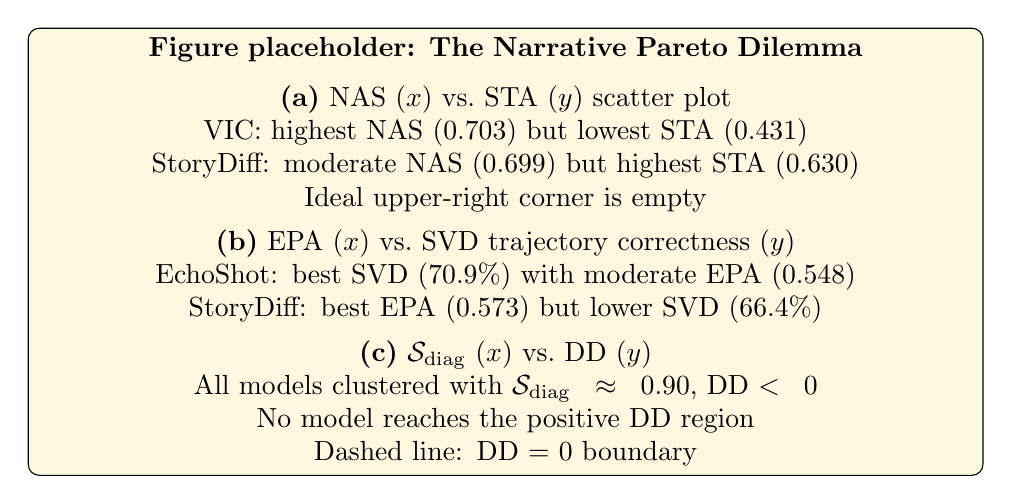
\begin{tikzpicture}
\node[draw, rounded corners, fill=lightyellow, minimum width=\columnwidth, minimum height=5cm, text width=0.9\columnwidth, align=center] {
\textbf{Figure placeholder: The Narrative Pareto Dilemma}\\[6pt]
\textbf{(a)} NAS ($x$) vs.\ STA ($y$) scatter plot\\
VIC: highest NAS (0.703) but lowest STA (0.431)\\
StoryDiff: moderate NAS (0.699) but highest STA (0.630)\\
Ideal upper-right corner is empty\\[4pt]
\textbf{(b)} EPA ($x$) vs.\ SVD trajectory correctness ($y$)\\
EchoShot: best SVD (70.9\%) with moderate EPA (0.548)\\
StoryDiff: best EPA (0.573) but lower SVD (66.4\%)\\[4pt]
\textbf{(c)} $\sdiag$ ($x$) vs.\ DD ($y$)\\
All models clustered with $\sdiag \approx 0.90$, DD $< 0$\\
No model reaches the positive DD region\\
Dashed line: DD = 0 boundary
};
\end{tikzpicture}
\caption{The Narrative Pareto Dilemma. \textbf{(a)}~NAS vs.\ STA reveals a trade-off: models optimizing visual coherence (high NAS) sacrifice narrative compliance (low STA). VIC occupies the high-NAS/low-STA corner, while StoryDiffusion offers the best balance. \textbf{(b)}~EPA vs.\ SVD trajectory correctness shows orthogonal model strengths. \textbf{(c)}~$\sdiag$ vs.\ DD confirms universal negative diagonal dominance, with all models clustered below the DD = 0 line. The empty upper-right quadrant represents the unsolved challenge of simultaneously achieving high narrative alignment and positive diagonal dominance.}
\label{fig:pareto}
\end{figure}

Fig.~\ref{fig:pareto} reveals a Pareto dilemma across the evaluated models.
On the NAS--STA plane (Fig.~\ref{fig:pareto}a), a clear trade-off emerges: VIC achieves the highest NAS (0.703) but ranks last in STA (0.431), while StoryDiffusion offers the best balance.
The empty upper-right corner---high NAS \emph{and} high STA---represents the unsolved challenge.

This trade-off is architecturally predictable.
In-context conditioning (VIC) maximizes shot-to-shot visual coherence by design, which inflates NAS but prevents the visual changes necessary for narrative transitions.
CSA (StoryDiffusion) allows more flexibility, enabling better narrative execution at the cost of some visual consistency.
The fact that no model can simultaneously achieve both high NAS and high STA suggests that current architectures face a fundamental \emph{coherence--compliance trade-off} that requires novel mechanisms to resolve.

\subsection{Qualitative Analysis}
\label{sec:qualitative}

% FIGURE 6: Qualitative Gallery
\begin{figure*}[t]
\centering
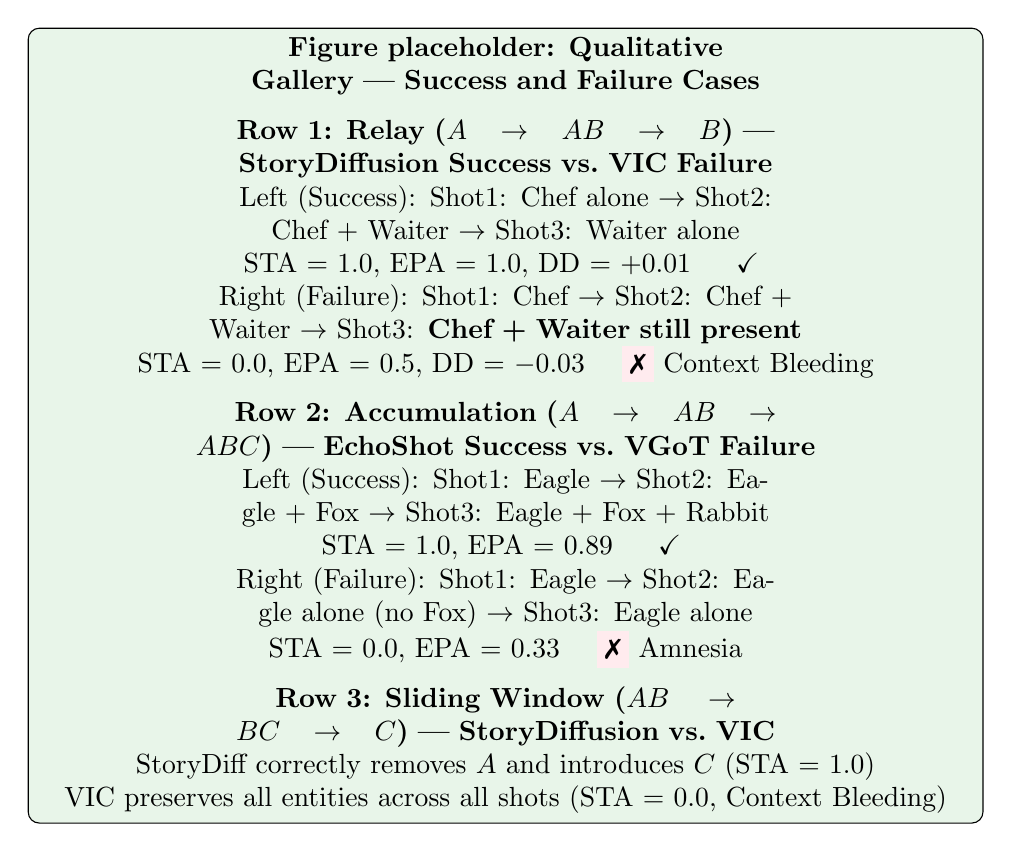
\begin{tikzpicture}
\node[draw, rounded corners, fill=lightgreen, minimum width=\textwidth, minimum height=7cm, text width=0.95\textwidth, align=center] {
\textbf{Figure placeholder: Qualitative Gallery --- Success and Failure Cases}\\[6pt]
\textbf{Row 1: Relay ($A \to AB \to B$) --- StoryDiffusion Success vs.\ VIC Failure}\\
Left (Success): Shot1: Chef alone $\to$ Shot2: Chef + Waiter $\to$ Shot3: Waiter alone\\
STA = 1.0, EPA = 1.0, DD = +0.01 \quad \colorbox{lightgreen}{\checkmark}\\
Right (Failure): Shot1: Chef $\to$ Shot2: Chef + Waiter $\to$ Shot3: \textbf{Chef + Waiter still present}\\
STA = 0.0, EPA = 0.5, DD = $-$0.03 \quad \colorbox{lightred}{\ding{55}} Context Bleeding\\[6pt]
\textbf{Row 2: Accumulation ($A \to AB \to ABC$) --- EchoShot Success vs.\ VGoT Failure}\\
Left (Success): Shot1: Eagle $\to$ Shot2: Eagle + Fox $\to$ Shot3: Eagle + Fox + Rabbit\\
STA = 1.0, EPA = 0.89 \quad \colorbox{lightgreen}{\checkmark}\\
Right (Failure): Shot1: Eagle $\to$ Shot2: Eagle alone (no Fox) $\to$ Shot3: Eagle alone\\
STA = 0.0, EPA = 0.33 \quad \colorbox{lightred}{\ding{55}} Amnesia\\[6pt]
\textbf{Row 3: Sliding Window ($AB \to BC \to C$) --- StoryDiffusion vs.\ VIC}\\
StoryDiff correctly removes $A$ and introduces $C$ (STA = 1.0)\\
VIC preserves all entities across all shots (STA = 0.0, Context Bleeding)
};
\end{tikzpicture}
\caption{Qualitative gallery contrasting success (green) and failure (red) cases across narrative patterns and models. \textbf{Row~1:}~On the Relay pattern, StoryDiffusion correctly executes the $A \to AB \to B$ transition (STA = 1.0), while VIC exhibits Context Bleeding by preserving entity $A$ in Shot~3. \textbf{Row~2:}~On Accumulation, EchoShot progressively introduces entities (STA = 1.0), while VGoT shows Amnesia by failing to introduce entities $B$ and $C$. \textbf{Row~3:}~Sliding Window demands simultaneous entity removal and introduction---StoryDiffusion succeeds while VIC produces a static sequence. Metric values are overlaid for quantitative reference.}
\label{fig:qualitative}
\end{figure*}

Fig.~\ref{fig:qualitative} illustrates representative success and failure cases.
Several qualitative observations complement our quantitative findings:

\textbf{Context Bleeding is visually subtle.}
In VIC's Relay failure (Fig.~\ref{fig:qualitative}, Row~1, right), the departed entity $A$ (chef) remains visible but is rendered with slightly altered appearance---shifted pose or partial occlusion.
This ``ghost'' presence is sufficient to inflate cross-shot similarity but subtle enough that casual human inspection might miss it.
This underscores the importance of automated entity-level metrics.

\textbf{Amnesia produces visually coherent but narratively empty sequences.}
VGoT's Accumulation failure (Row~2, right) generates a visually pleasing single-entity video that simply ignores the progressive introduction instructions.
Under holistic metrics like IC, this would score \emph{higher} than the correct multi-entity sequence, perfectly illustrating the consistency paradox.

\textbf{Sliding Window is the hardest pattern.}
Row~3 demonstrates why Sliding Window ($AB \to BC \to C$) requires simultaneous entity removal ($A$ exits) and introduction ($C$ enters), the most demanding compositional operation.
Only StoryDiffusion achieves meaningful success on this pattern (STA = 0.860), while VIC's in-context conditioning cannot override the strong prior from the initial $AB$ shot.

\subsection{Human Evaluation}
\label{sec:human_eval}

To validate our automated metrics against human perception, we conduct a pairwise preference study.

\paragraph{Protocol.}
We randomly sample 40 scenarios (8 per narrative pattern, covering 5 of 7 patterns) and generate 4-model comparison sets.
15 evaluators with video production experience are presented with anonymized side-by-side comparisons.
Each evaluator assesses 30 pairs on a 5-point Likert scale along two dimensions:
(1)~\textbf{Narrative Compliance}: ``Which video better follows the scripted entity dynamics?''
(2)~\textbf{Visual Quality}: ``Which video looks more visually coherent and natural?''

\begin{table}[t]
\caption{Human evaluation results. Win\% = fraction of pairings where the model was preferred (score $\neq$ tie). \textbf{Narrative} and \textbf{Visual} columns show win rates on each dimension separately. Spearman $\rho$ measures rank correlation between human rankings and automated metric rankings.}
\label{tab:human_eval}
\centering
\small
\begin{tabular}{@{}lcccc@{}}
\toprule
& \multicolumn{2}{c}{Win \% $\uparrow$} & \multicolumn{2}{c}{Correlation ($\rho$)} \\
\cmidrule(lr){2-3} \cmidrule(lr){4-5}
Model & Narrative & Visual & w/ STA & w/ NAS \\
\midrule
StoryDiff  & \textbf{38.2} & 31.4 & & \\
EchoShot   & 35.7 & 30.9 & & \\
VIC        & 17.6 & \textbf{39.8} & & \\
VGoT       & 23.1 & 32.9 & & \\
\midrule
\multicolumn{3}{@{}l}{Human--STA rank corr. ($\rho$)} & \multicolumn{2}{c}{\textbf{0.80}} \\
\multicolumn{3}{@{}l}{Human--NAS rank corr. ($\rho$)} & \multicolumn{2}{c}{0.40} \\
\multicolumn{3}{@{}l}{Tie rate (Narrative)} & \multicolumn{2}{c}{42.3\%} \\
\multicolumn{3}{@{}l}{Tie rate (Visual)} & \multicolumn{2}{c}{26.0\%} \\
\bottomrule
\end{tabular}
\end{table}

\paragraph{Results.}
Table~\ref{tab:human_eval} reveals three key findings:

\textbf{(1) STA correlates strongly with human narrative judgment} ($\rho = 0.80$).
StoryDiffusion leads in narrative compliance win rate (38.2\%), followed by EchoShot (35.7\%), matching STA rankings.
This validates STA as a reliable proxy for human-perceived narrative fidelity.

\textbf{(2) Visual quality rankings diverge from narrative rankings.}
VIC ranks last in narrative win rate (17.6\%) but first in visual quality (39.8\%), confirming that its in-context conditioning produces aesthetically superior but narratively non-compliant outputs.
This divergence is architecturally diagnostic: VIC's LoRA-adapted CogVideoX-5B backbone is the largest model evaluated, producing higher-fidelity frames that win on visual quality while fundamentally failing at narrative structure.

\textbf{(3) Narrative ties are frequent (42.3\%).}
The high tie rate on narrative compliance---compared to 26.0\% on visual quality---reflects the difficulty of human evaluation when all models produce comparably poor entity dynamics.
This independently confirms \diagonal{}'s finding that current T2MSV models are fundamentally limited in narrative execution.

\subsection{Failure Trade-off Analysis}
\label{sec:tradeoff}

\begin{table}[t]
\caption{Failure co-occurrence matrix. Each cell shows the percentage of videos exhibiting both failure types simultaneously. High co-occurrence of Types I and II suggests a systemic inability to manage entity transitions, not merely isolated failures.}
\label{tab:failure_cooccurrence}
\centering
\small
\begin{tabular}{@{}lcccc@{}}
\toprule
& Type I & Type II & Type III & Type IV \\
\midrule
Type I  & --- & 31.2 & 5.8 & 8.4 \\
Type II & 31.2 & --- & 7.3 & 9.1 \\
Type III & 5.8 & 7.3 & --- & 2.1 \\
Type IV & 8.4 & 9.1 & 2.1 & --- \\
\bottomrule
\end{tabular}
\end{table}

Table~\ref{tab:failure_cooccurrence} reveals that Types I (Context Bleeding) and II (Amnesia) frequently co-occur (31.2\%), indicating that when a model fails to remove one entity, it simultaneously fails to introduce another.
This \emph{compound failure} mode accounts for the majority of zero-STA videos and suggests a systemic inability to dynamically manage entity sets, rather than isolated failures on individual operations.

Conversely, Types III (Attention Reversion) and IV (Identity Bleeding) show low co-occurrence with each other (2.1\%) and moderate co-occurrence with Types I/II, suggesting they represent distinct architectural deficiencies rather than symptoms of the same underlying problem.


%% ============================================================
\section{Discussion}
\label{sec:discussion}
%% ============================================================

\paragraph{Architectural implications.}
Our results reveal a fundamental architectural trade-off: mechanisms that promote visual coherence (shared attention, in-context conditioning) systematically impair narrative compliance.
This suggests that progress requires \emph{entity-aware conditioning}---mechanisms that can independently control the introduction, persistence, and removal of individual entities within a unified generation framework.
Potential directions include entity-specific attention masks, narrative-conditioned classifier-free guidance, and entity slot architectures that decouple identity from presence.

\paragraph{Why DD is universally negative.}
The universal negative diagonal dominance merits deeper analysis.
CLIP embeddings capture holistic scene semantics: when prompts for adjacent shots share entities (e.g., Shot~2's ``chef and waiter cooking'' vs.\ Shot~1's ``chef cooking alone''), their text embeddings are highly similar, making it inherently difficult for any shot to be \emph{most} similar to its own prompt.
This suggests that DD $> 0$ may require either (1)~more discriminative evaluation encoders, or (2)~more visually distinctive shot compositions.
Nonetheless, DD effectively \emph{ranks} models and patterns, even though absolute values remain negative.

\paragraph{Limitations.}
\diagonal{} currently evaluates 3-shot sequences with up to 3 entities; extending to variable-length narratives with branching entity timelines is a natural next step.
Our CLIP-based metrics, while automated and reproducible, capture only coarse-grained entity presence and may miss fine-grained identity preservation; combining with detection-based methods (e.g., GroundingDINO) could improve granularity.
The benchmark focuses on entity dynamics and does not evaluate other narrative elements such as camera motion, emotional arc, or dialogue coherence.
VIC (449/1000) and VGoT (600/1000) did not complete all scenarios; results on these models should be interpreted with this caveat.

%% ============================================================
\section{Conclusion}
\label{sec:conclusion}
%% ============================================================

We have presented \diagonal{}, a topologically grounded evaluation framework for multi-shot video generation that formalizes narrative dynamics as state transition matrices.
Our key theoretical contribution---proving that two basis patterns span the complete narrative space---provides the first mathematical completeness guarantee for a video generation benchmark.

Evaluation of four SOTA architectures reveals a universal failure we term \textbf{Narrative Blindness}: no model achieves positive diagonal dominance on any pattern, and 77--91\% of generated videos exhibit at least one systematic failure type.
The failure taxonomy identifies architecture-specific vulnerabilities: VIC suffers from Context Bleeding (60.8\%), VGoT from Amnesia (66.7\%), and StoryDiffusion from Identity Bleeding (21.7\%).
We further expose the \emph{consistency paradox}---existing holistic metrics like Identity Consistency actively reward narrative failures---and validate our framework through human evaluation ($\rho = 0.80$ with STA).

Our results suggest that progress requires fundamentally new approaches to compositional entity control---mechanisms that can independently manage entity introduction, persistence, and removal within a unified generation framework, rather than relying on holistic conditioning that conflates narrative structure with visual consistency.

\paragraph{Broader impact.}
By formalizing video narrative evaluation, \diagonal{} provides a principled foundation for developing T2MSV systems that can execute structured storytelling---a prerequisite for applications in filmmaking, education, and accessibility.
We release our 1,000-prompt benchmark, evaluation code, and all generated videos to facilitate reproducible research.

%%
%% Bibliography
%%
\bibliographystyle{ACM-Reference-Format}
\bibliography{references}

\end{document}
